% Latex template: mahmoud.s.fahmy@students.kasralainy.edu.eg
% For more details: https://www.sharelatex.com/learn/Beamer

\documentclass[aspectratio=1610]{beamer}					% Document class

\setbeamertemplate{footline}[text line]{%
  \parbox{\linewidth}{\vspace*{-8pt}Dynamics on gene networks \hfill\insertshortauthor\hfill\insertpagenumber}}
\setbeamertemplate{navigation symbols}{}

\usepackage[english]{babel}				% Set language
\usepackage[utf8x]{inputenc}			% Set encoding

\mode<presentation>						% Set options
{
  \usetheme{default}					% Set theme
  \usecolortheme{default} 				% Set colors
  \usefonttheme{default}  				% Set font theme
  \setbeamertemplate{caption}[numbered]	% Set caption to be numbered
}

% Uncomment this to have the outline at the beginning of each section highlighted.
%\AtBeginSection[]
%{
%  \begin{frame}{Outline}
%    \tableofcontents[currentsection]
%  \end{frame}
%}

\usepackage{graphicx}					% For including figures
\usepackage{booktabs}					% For table rules
\usepackage{hyperref}	
\usepackage{tikz-network}				% For cross-referencing
\usepackage[absolute,overlay]{textpos}
\usepackage{bm}
\usepackage[font=small,labelfont=bf]{caption}

\title{Isolating the perturbation response of gene regulatory networks in the presence of biological variability and technical noise}	% Presentation title
\author{Clayton W. Seitz}								% Presentation author
\date{\today}									% Today's date	

\begin{document}

% Title page
% This page includes the informations defined earlier including title, author/s, affiliation/s and the date
\begin{frame}
  \titlepage
\end{frame}

% The following is the most frequently used slide types in beamer
% The slide structure is as follows:
%
%\begin{frame}{<slide-title>}
%	<content>
%\end{frame}

\begin{frame}{Drug-induced
reprogramming as a mode of cancer drug resistance}

\begin{textblock*}{12cm}(2cm,1cm)
\begin{figure}
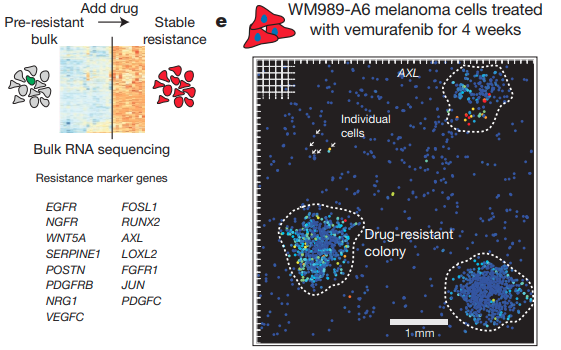
\includegraphics[width=12cm]{resistance.png}
\caption{Shaffer et al., Nature 2017}
\end{figure}
\end{textblock*}

\end{frame}

\begin{frame}{WM989-A6 RNA-FISH data summary}

\begin{textblock*}{15cm}(0.5cm,1cm)
\begin{figure}
\includegraphics[width=15cm]{data-summary.png}
\end{figure}
\end{textblock*}

\end{frame}

\begin{frame}{Graphical abstract}

\begin{textblock*}{14cm}(1.15cm,1.5cm)
\begin{figure}
\captionsetup{font={footnotesize,it}}
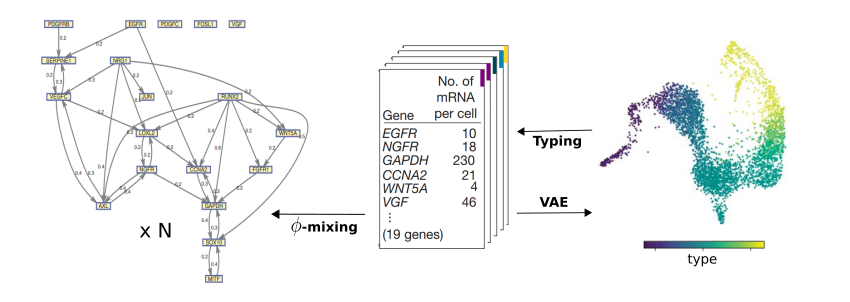
\includegraphics[width=14cm]{sketch.png}
\caption{Gene expression matrices used as training data to learn a latent-space representation of gene expression, uncovering latent structure of the joint distribution and permitting cell typing, account for batch variability. Type information is then used for inference of the underlying regulatory network using the phi-mixing coefficient, which may differ across types}
\end{figure}
\end{textblock*}

\end{frame}

\begin{frame}{Modeling stochastic biochemical reaction networks}

\begin{textblock*}{15cm}(0.5cm,1.5cm)
Three ways of representing a biochemical reaction network:
\end{textblock*}

\begin{textblock*}{15cm}(0.5cm,2cm)
\begin{center}
\noindent\begin{minipage}{.3\linewidth}
\begin{center}
\begin{align*}
r_{1}&: x_{1} + x_{2} \rightarrow x_{3}\\
r_{2}&: x_{3} + x_{4} \rightarrow 2x_{3}\\
r_{3}&: x_{4} + x_{5} \rightarrow x_{2}
\end{align*}
\end{center}
\end{minipage}%
\begin{minipage}{.3\linewidth}
\begin{center}
\begin{align*}
\mathbf{\nu} = \begin{pmatrix}
-1 & -1 & 1 & 0 & 0\\
0 & 0 & 1 & 1 & 0\\
0 & 1 & 0 & -1 & -1\\
\end{pmatrix}
\end{align*}
\end{center}
\end{minipage}
\begin{minipage}{.3\linewidth}
\begin{center}
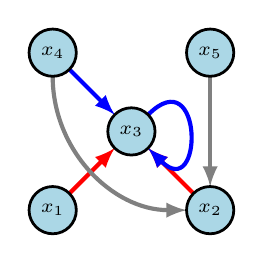
\begin{tikzpicture}
\Vertex[label=$x_{1}$]{A}
\Vertex[x=2,label=$x_{2}$]{B}
\Vertex[x=1,y=1,label=$x_{3}$]{C}
\Vertex[x=0,y=2,label=$x_{4}$]{D}
\Vertex[x=2,y=2,label=$x_{5}$]{E}
\Edge[Math,Direct=true,color=red](A)(C)
\Edge[Math,Direct=true,color=red](B)(C)
\Edge[Math,Direct=true,color=blue](C)(C)
\Edge[Math,Direct=true,color=blue](D)(C)
\Edge[Math,Direct=true,bend=-45,color=gray](D)(B)
\Edge[Math,Direct=true,color=gray](E)(B)
\end{tikzpicture}
\end{center}
\end{minipage}
\end{center}
\end{textblock*}

\end{frame}

\begin{frame}{Bayesian parameter inference for gene regulation}

Suppose we 

\end{frame}

\begin{frame}{Training on BBBC039 U2OS Cells}
\vspace{0.1in}
BBBC039: 200 images, 160 train + 40 validation, 256\;x\;256 random crop

\begin{center}
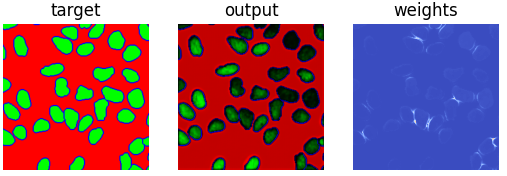
\includegraphics[width=0.8\textwidth]{weights.png}
\end{center}

We train a 3-channel semantic segmentation model with \textbf{weighted} cross-entropy loss:

\begin{equation*}
\mathcal{L} = \sum_{i,j} w_{ij}\log p_{ij}(\tilde{x}) = \sum_{i,j} w_{ij}\log \frac{\exp(-s_{ij}(\tilde{x}))}{\sum_{x\in\chi} \exp(-s_{ij}(\tilde{x}))}
\end{equation*}

$p_{ij}$ is the probability the model assigns a pixel to the true class $\tilde{x} \in \{\textrm{a}, \textrm{b}, \textrm{c}\}$

\end{frame}

\begin{frame}{Training on BBBC039 U2OS Cells}

\begin{center}
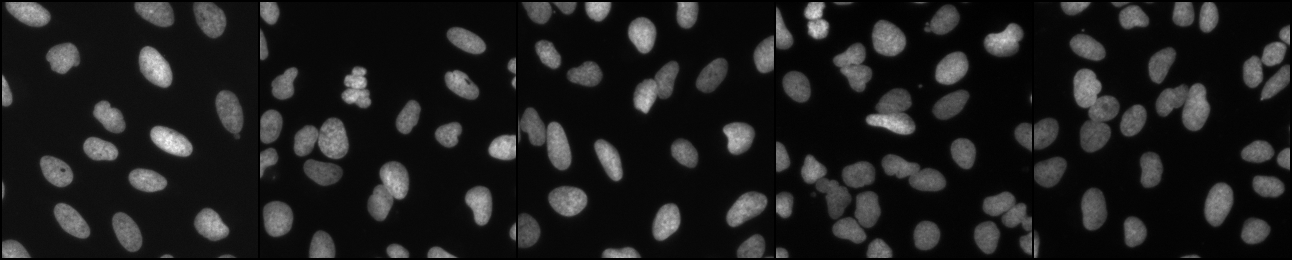
\includegraphics[width=0.85\textwidth]{input-train.png}
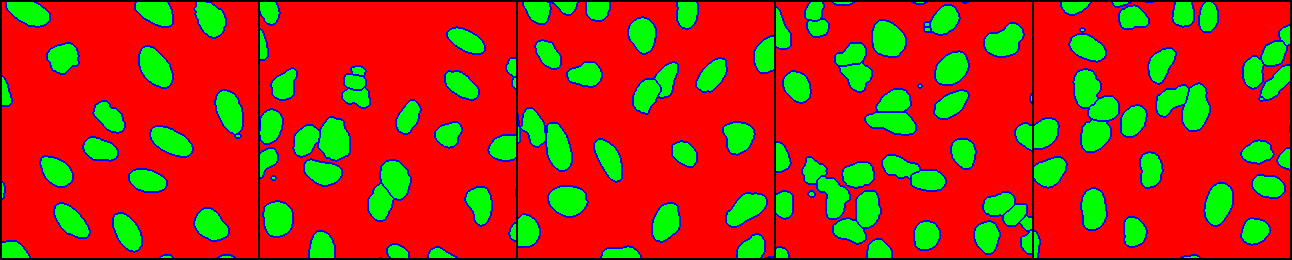
\includegraphics[width=0.85\textwidth]{target-train.png}
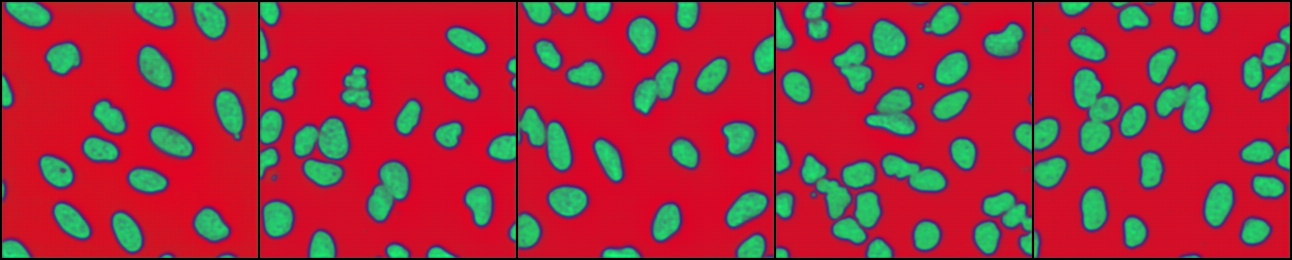
\includegraphics[width=0.85\textwidth]{output-train.png}
\end{center}

\end{frame}

\begin{frame}{Training on BBBC039 U2OS Cells}
Learning rate $\eta=0.01$, Batch-size $B=5$ (32 train iterations, 8 validation)
\begin{center}
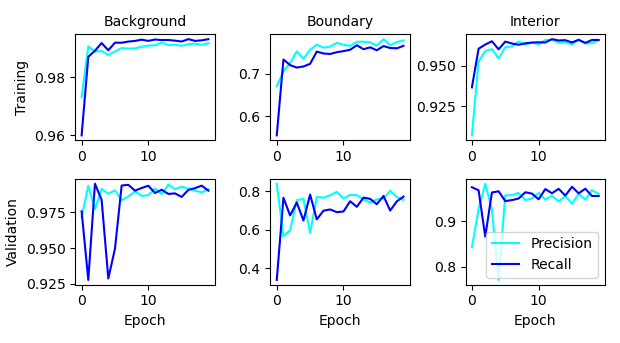
\includegraphics[width=0.85\textwidth]{metrics.png}
\end{center}

\end{frame}



% Adding the option 'allowframebreaks' allows the contents of the slide to be expanded in more than one slide.
\begin{frame}[allowframebreaks]{References}
	\tiny\bibliography{references}
	\bibliographystyle{apalike}
\end{frame}

\end{document}
